\documentclass{article}
\usepackage{graphicx} % Required for inserting images
\usepackage[margin=1in]{geometry}
\usepackage{amsmath}
\usepackage{amsthm}
\usepackage{amssymb}
\usepackage{amsfonts}
\usepackage{enumitem}
\usepackage{verbatim}
\usepackage{xcolor}
\usepackage{soul}

\title{Homework 3: Report}
\author{Dante Buhl}

\DeclareMathOperator{\cond}{cond}
\DeclareMathOperator{\vecspan}{span}

\begin{document}

\newcommand{\bs}[1]{\boldsymbol{#1}}
\newcommand{\bmp}[1]{\begin{minipage}{#1\textwidth}}
\newcommand{\emp}{\end{minipage}}
\newcommand{\R}{\mathbb{R}}
%\newcommand{\Imag}{\mathbb{I}}
\newcommand{\C}{\mathbb{C}}
\newcommand{\N}{\mathcal{N}}
\newcommand{\I}{\mathrm{I}}
\newcommand{\K}{\bs{\mathrm{K}}}
\newcommand{\m}{\bs{\mu}_*}
\newcommand{\s}{\bs{\Sigma}_*}
\newcommand{\dt}{\Delta t}
\newcommand{\dx}{\Delta x}
\newcommand{\tr}[1]{\text{Tr}(#1)}
\newcommand{\Tr}[1]{\text{Tr}(#1)}
\newcommand{\pd}[2]{\frac{\partial #1}{\partial #2}}

\maketitle

\section*{Question 1: Consistency and Stability}
    \begin{align}
        \begin{cases}
            U_t + U_x = 0 \quad \quad x \in [0, 2\pi],
            \quad t \ge 0\\
            U(x,0) = \sin^2(x)\\
            \text{Periodic B.C.}
        \end{cases} \\
        u_j^{k+1} = u_j^k - \frac{\dt}{2\dx}(u_{j+1}^{k+1} - u_{j-1}^{k+1})
    \end{align}

\begin{enumerate}[label=\alph*)]

    \item Compute the Local Truncation Error of the scheme in (2). Is the scheme
    consistent? If so, to which orders in $\dt$ and $\dx$
    \begin{proof}
        \begin{align*}
            \dt \tau_j^{k+1} &= \bs{y}_j^{k+1} - \bs{y}_j^k + \frac{\dt}{2\dx}(\bs{y}_{j+1}^{k+1}
            - \bs{y}_{j-1}^{k+1})\\
            \tau_j^{k+1} &= \dot{\bs{y}}_j^{k+1} + \frac{\dt}{2}\ddot{\bs{y}}_j^{k+1} +
            O(\dt^2) + 
            \frac{1}{2\dx}(2\dx \bs{y}_{x j}^{k+1} + \frac{2\dx^3}{6} \bs{y}_{x j}^{k+1}
            +O(\dx^5))\\
            \tau_j^{k+1} &= \frac{\dt}{2}\ddot{\bs{y}}_j^{k+1} +
            \frac{\dx^2}{6} \bs{y}_{xxx j}^{k+1} + O(\dt^2)+O(\dx^4) 
        \end{align*}
        Thus we have shown that the local truncation error, $\tau_j^{k+1}$
        scales with $\dt$ with order 1, and with $\dx$ with order 2. Thus, the
        scheme is consistent with order 1 in time and order 2 in space. 
    \end{proof}

    \item Compute the Von-Neumann Stability Analysis of (2). Is the scheme
    convergent?
    \begin{proof}
        There are two methods to show that this method is stable. We can show
        this wih Lax-Richtmyer stability or with Von Neumann stability theory.
        First, we can show rather easily, 
        \begin{align*}
            u^{k+1} (\I + \dt D1_{PFD2}) = u^{k}\\
            u^{k+1} =  (\I + \dt D1_{PFD2})^{-1} u^{k}\\
            B = (\I + \dt D1_{PFD2})^{-1}
        \end{align*}
        We can consider the eigenvalues of $B^{-1}$ which are not difficult to
        compute and show rather easily that the spectral radius of B has an
        upper bound of 1. Note that $D1_{PFD2}$ is the periodic first differentiation
        matrix for second ordered finite differences. This looks like the following logic,
        \begin{align*}
            \det(\I(1-\lambda) + \dt D1_{PFD2}) = (1 -\lambda)^N +
            \frac{\dt}{2\dx}((-1)^N + 1)\\
            \lambda = 1 \mp \sqrt[N]{-\frac{\dt}{2\dx}((-1)^N + 1)}
        \end{align*}
        Obviously this produces eigenvalues all of which are larger than 1 in
        magnitude. Thus we can use some logic from linear algebra finding that
        the eigenvalues of an inverse matrices are the multiplicative inverses
        of the eigenvalues of the original matrix. That is, we have bounded the
        eigenvalues of the transformation with a spectral radius of less than 1
        and have proved stability. However, the von neumann method is analogous.

        We use the substitution $u_j^k = c_p^ke^{ijp\xi}$. 
        \begin{align*}
            c_p^{k+1}(1 + \frac{\dt}{2\dx}(e^{ip\xi} - e^{-ip\xi})) = c_p^k\\
            c_p^{k+1}(1 + i\frac{\dt}{\dx}\sin(p\xi)) = c_p^k\\
            c_p^{k+1} = \frac{1}{1 + i\frac{\dt}{\dx}\sin(p\xi)}c_p^k\\
            \frac{1}{1 + i\frac{\dt}{\dx}\sin(p\xi)} = \frac{1 - i\frac{\dt}{\dx}\sin(p\xi)}{1 +
            \frac{\dt^2}{\dx^2}\sin^2(p\xi)}\\
            \left|\frac{1}{1 + i\frac{\dt}{\dx}\sin(p\xi)}\right| = \frac{\sqrt{1 +
            \frac{\dt^2}{\dx^2}\sin^2(p\xi)}}{1 +
            \frac{\dt^2}{\dx^2}\sin^2(p\xi)} \le 1
        \end{align*}
        Therefore we have shown using Von Neumann stability theory that the
        scheme is stable. Since we have coupled stability and consistency we
        have convergence with order 1 in $\dt$ and order 2 in $\dx$. 
    \end{proof}
\end{enumerate}

\section*{Question 2: Method of Characteristics for Advection}\
    \large
    \begin{align}
        \begin{cases}
            U_t + (fU)_x + (gU)_y =0 \\
            U(x,y,0) = \frac{1}{2\pi^2}\sin^2(x+y)
        \end{cases}
    \end{align}
    \normalsize
    \begin{align}
        f(x,y) = \sin(x)\sin(y), \quad\quad g(x,y) = 1 - e^{\sin(x+y)} \\
        \mathbb{T} = \left\{(x,y) \in \R^2:\quad 0 \le x \le 2\pi, \quad 0 \le
        y \le 2\pi\right\}
    \end{align}
    \begin{align}
        \begin{cases}
            U(0,y,t) = U(2\pi,y,t), \quad 0 \le y \le 2\pi\\
            U(x,0,t) = U(x,2\pi,t), \quad 0 \le x \le 2\pi
        \end{cases}
    \end{align}
\begin{enumerate}[label=\alph*)]

    \item Show that the following integral evaluates to 1. 
    \begin{align*}
        \int_{\mathbb{T}} U(x,y,t)dxdy = 1,\quad  \forall t \ge 0
    \end{align*}
    \begin{proof}
        \begin{align*}
            U_t &= -(fU)_x - (gU)_y \\
            \int_{\mathbb{T}} U_t dA &= \int_{\mathbb{T}}-(fU)_x - (gU)_y dA\\
            \pd{}{t}\int_{\mathbb{T}} U dA &= \int_{\mathbb{T}}-(fU)_x - (gU)_y dA\\
            \pd{}{t}\int_{\mathbb{T}} U dA &= \int_{\partial\mathbb{T}} -\left<fU,
            gU\right>\cdot \eta ds\\
            \eta &= 
            \begin{cases}
                \left<0,1\right>, y = 2\pi\\
                \left<0,-1\right>, y = 0\\
                \left<1,0\right>, x = 2\pi\\
                \left<-1,0\right>, x = 0
            \end{cases}
        \end{align*}
        \begin{align*}
            \pd{}{t}\int_{\mathbb{T}} U dA &= \int_0^{2\pi} fU|_{x=0} dy
            - \int_0^{2\pi} gU|_{y=2\pi} dx 
            - \int_0^{2\pi} fU|_{x=2\pi} dy
            + \int_0^{2\pi} gU|_{y=0} dx \\
        \end{align*}
        \begin{align*}
            \int_0^{2\pi} gU|_{y=0} dx &= \int_0^{2\pi} gU|_{y=2\pi} dx\\
            \int_0^{2\pi} fU|_{x=0} dy &= 0 \\
            \int_0^{2\pi} fU|_{x=2\pi} dy &= 0\\ 
            \pd{}{t}\int_{\mathbb{T}} U dA &= 0 
        \end{align*}
        Therefore we have that the value of the integral is constant. Now we
        must simply show that it is at one timestep equal to one. 
        \begin{align*}
            \int_{\mathbb{T}} U(x,y,0) dA &=
            \frac{1}{2\pi^2}\int_0^{2\pi}\int_0^{2\pi} \sin^2(x+y)dxdy\\
            &= \frac{1}{4\pi^2}\int_0^{2\pi}\int_0^{2\pi}1 - \cos(2x+2y)dxdy\\
            &= \frac{1}{4\pi^2}\left(4\pi^2 -
            \int_0^{2\pi}\int_0^{2\pi}\cos(2x+2y)dxdy\right)\\
            &= 1 - \frac{1}{4\pi^2}\int_0^{2\pi}\int_0^{2\pi}\cos(2x+2y)dxdy\\
            &= 1 - \frac{1}{4\pi^2}\int_0^{2\pi}0dxdy\\
            &= 1
        \end{align*}
        Thus we have that U will satisfy this integral at every timestep.
    \end{proof}
    
    \item See figure 1.
    \begin{figure}
        \centering
        \bmp{1}
            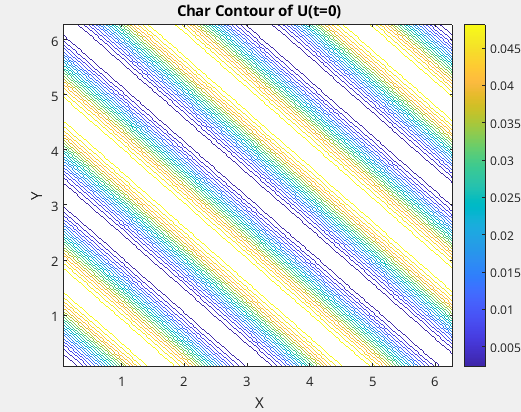
\includegraphics[width=0.32\textwidth]{t0charcontour.png}
            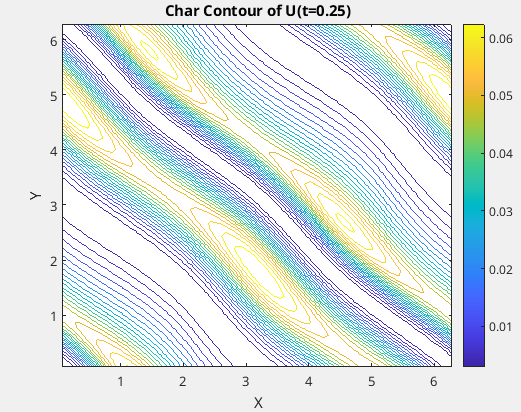
\includegraphics[width=0.32\textwidth]{t25charcontour.png}
            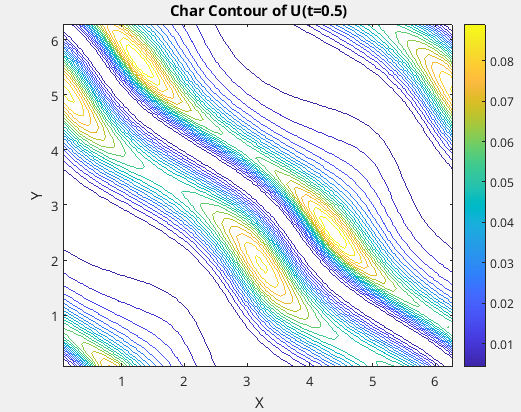
\includegraphics[width=0.32\textwidth]{t5charcontour.png}
        \emp

        \bmp{1}
            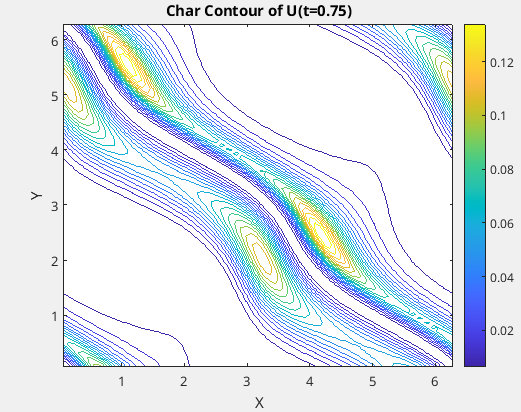
\includegraphics[width=0.32\textwidth]{t75charcontour.png}
            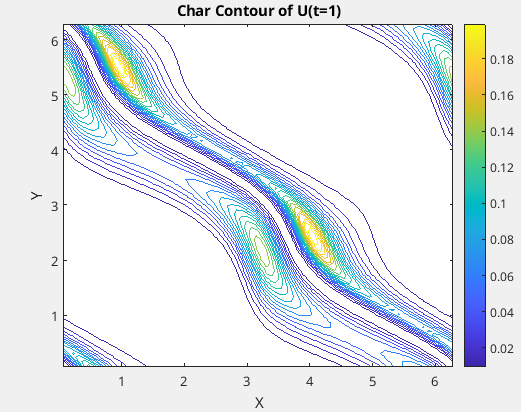
\includegraphics[width=0.32\textwidth]{t1charcontour.png}
            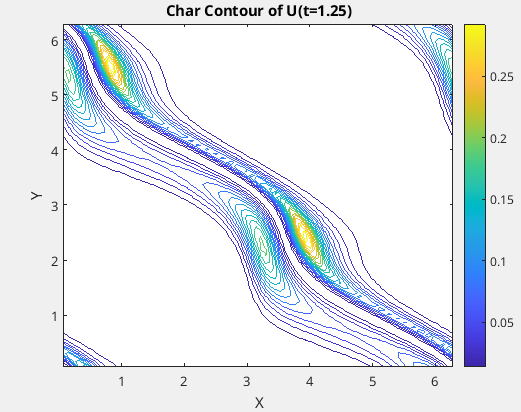
\includegraphics[width=0.32\textwidth]{t125charcontour.png}
        \emp
        \caption{Contour Plots of Solution using Method of Characteristics}
    \end{figure}

\end{enumerate}

\section*{Question 3: Finite Differences for Advection}

\begin{enumerate}[label=\alph*)]

    \item See figure 2.
    \begin{figure}
        \centering
        \bmp{1}
            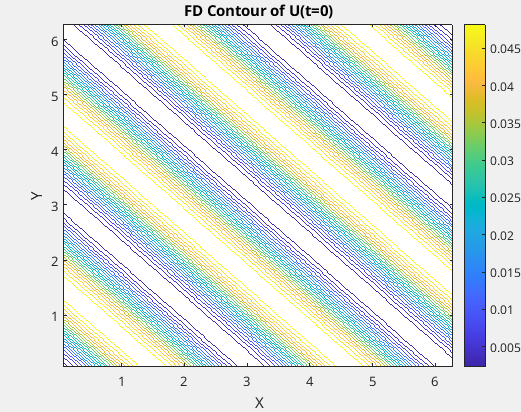
\includegraphics[width=0.32\textwidth]{t0fdcontour.png}
            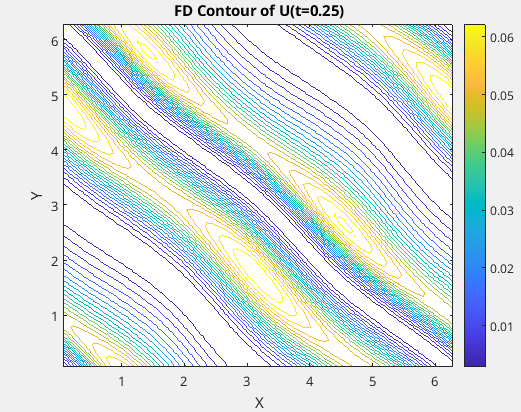
\includegraphics[width=0.32\textwidth]{t25fdcontour.png}
            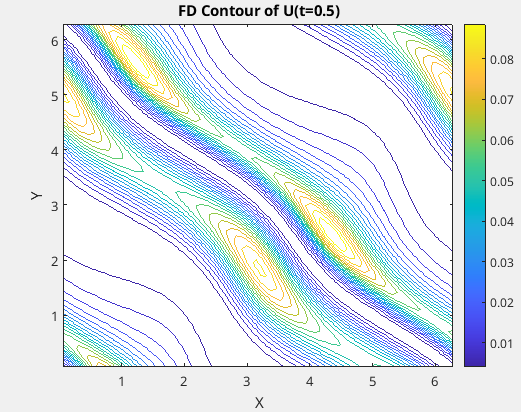
\includegraphics[width=0.32\textwidth]{t5fdcontour.png}
        \emp

        \bmp{1}
            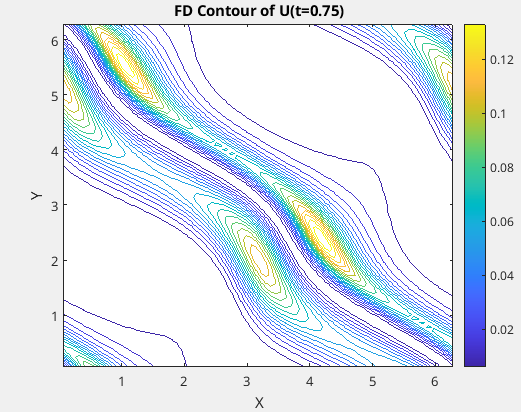
\includegraphics[width=0.32\textwidth]{t75fdcontour.png}
            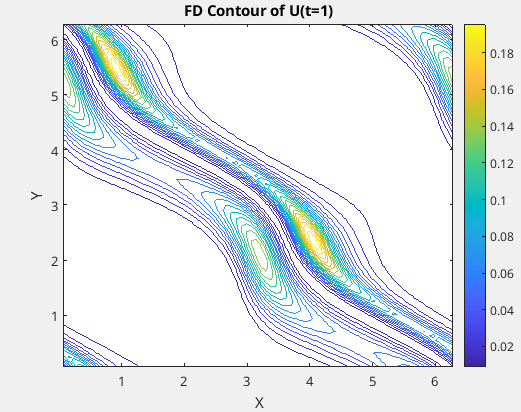
\includegraphics[width=0.32\textwidth]{t1fdcontour.png}
            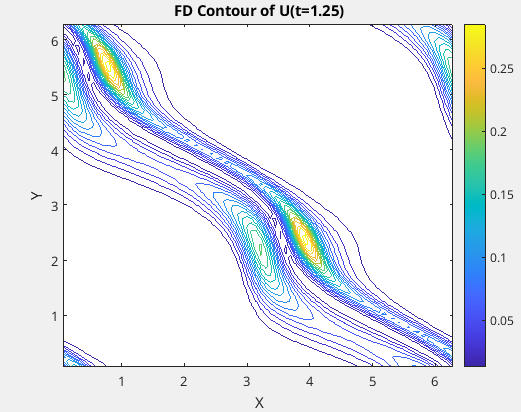
\includegraphics[width=0.32\textwidth]{t125fdcontour.png}
        \emp
        \caption{Contour Plots of Solution using Finite Differences}
    \end{figure}
    \item Yes! The discrete integral is constant up to numerical precision as we
    would expect (this is hard to see in the plot but if you look at fdint.dat
    after running the code it is clear that this is true). 
    \begin{figure}
        \centering
        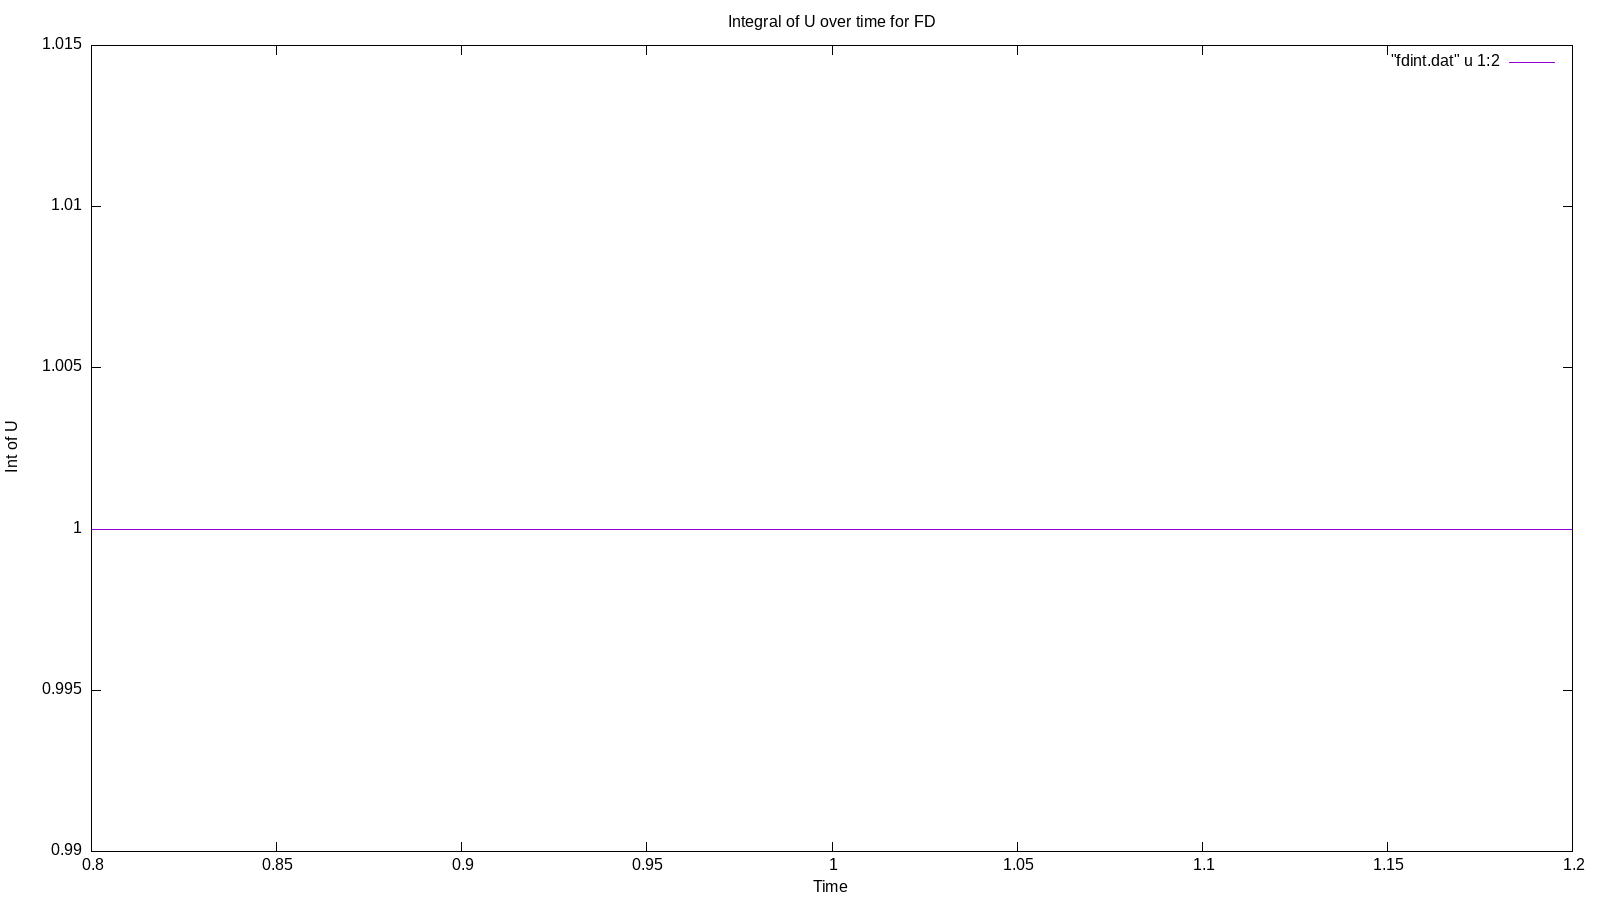
\includegraphics[width=0.9\textwidth]{fdi.png}
        \caption{Area Integral of Solution over Time}
    \end{figure}
   
    \item See figure 4.
     \begin{figure}
        \centering
        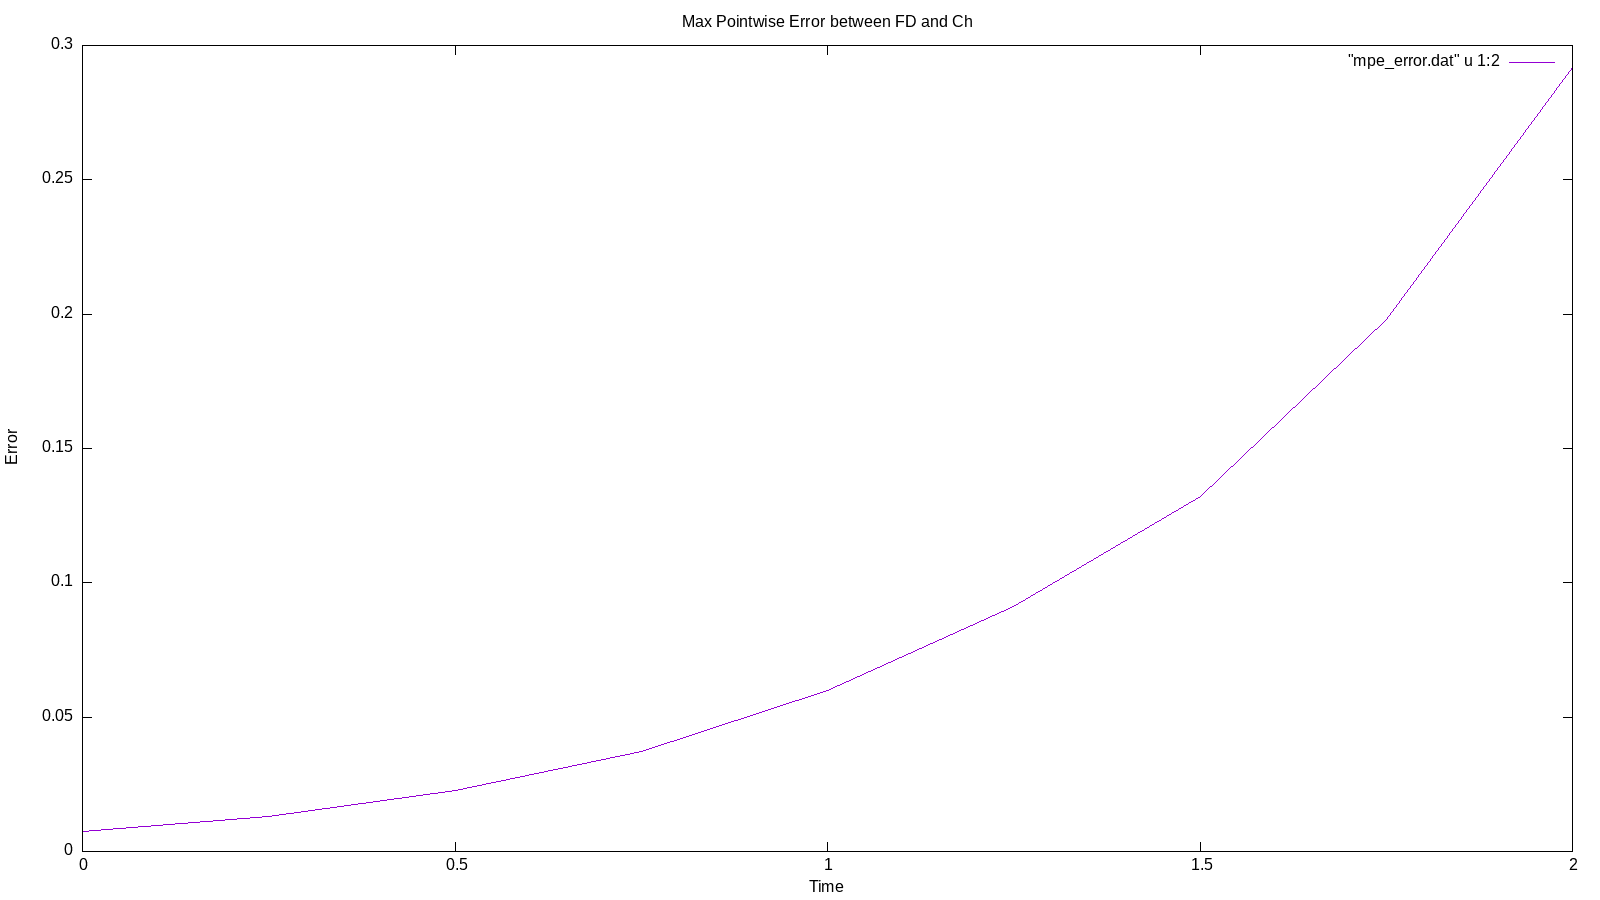
\includegraphics[width=0.9\textwidth]{mpe.png}
        \caption{Plot of Max Pointwise Error as a function of time}
    \end{figure}
       
    \item See figure 5. The MSE descreases with $N$. The order of decay seems to
    be quadratic after comparing the slope to that of a quadratic decay. This
    seems good! It is also important to consider that this plot is only as
    accurate as the combined accuracy of the method of Characteristics and
    finite differences combined. After fitting a line to the plot, a line of
    best fit seems to yield and order 2 decay!
    \begin{figure}
        \centering
        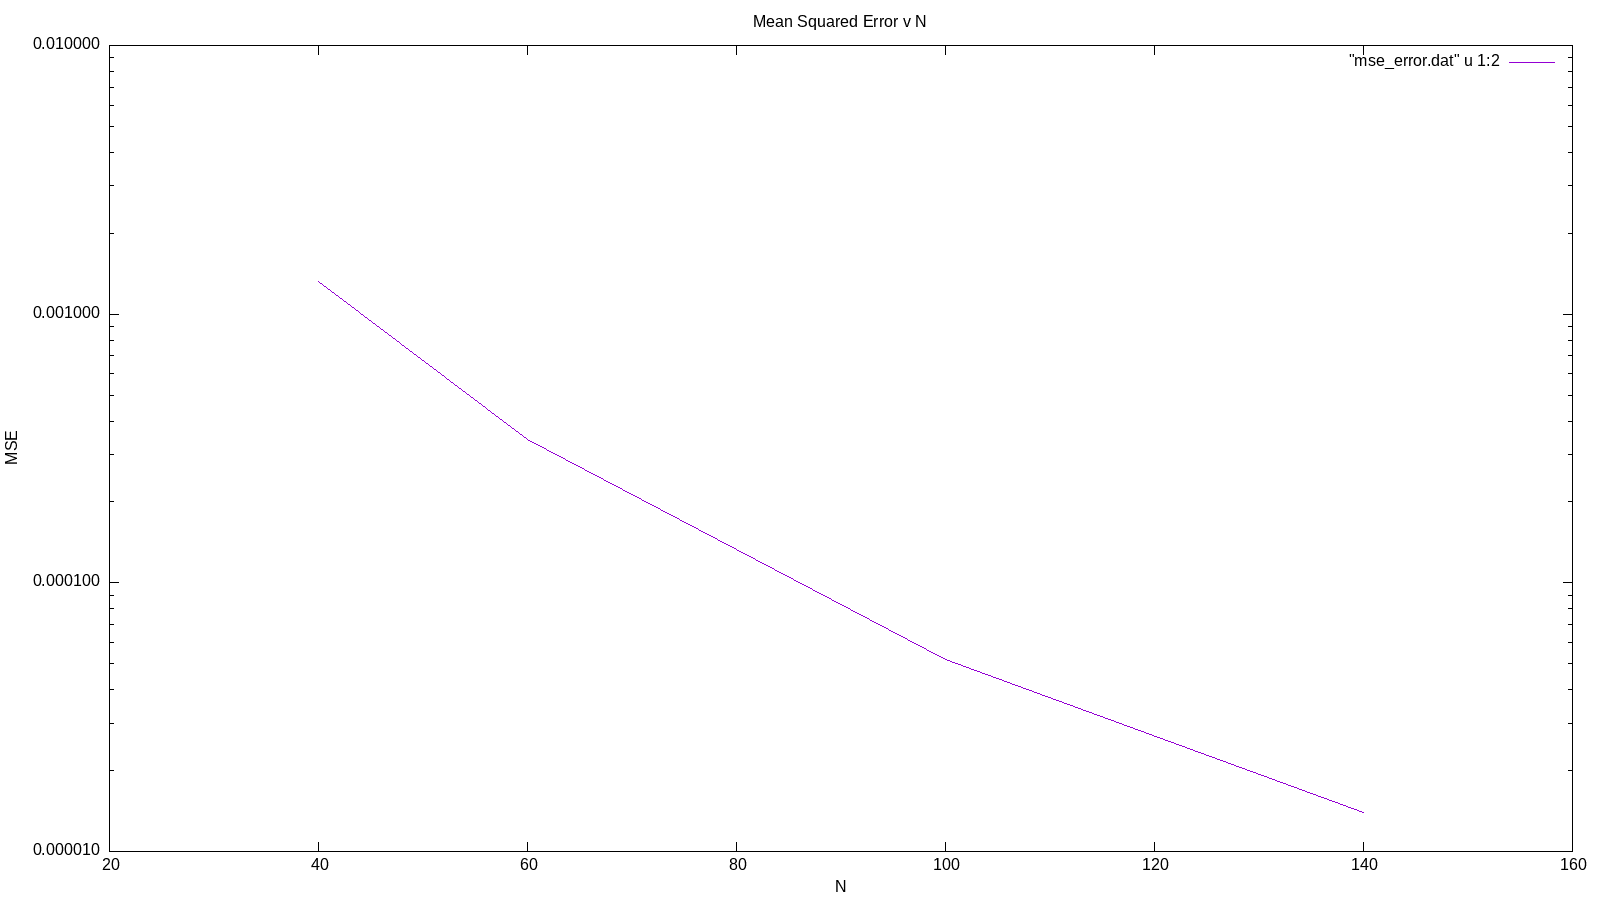
\includegraphics[width=0.9\textwidth]{mse.png}
        \caption{Plot of Mean Square Error as a function of gridsize}
    \end{figure}



\end{enumerate}

\end{document}
